\documentclass[letterpaper]{article}
\usepackage{natbib}
\usepackage[utf8]{inputenc}
\usepackage{graphicx}
\usepackage{color}
\usepackage{multirow}
\usepackage{amsmath}
\usepackage{array}
\usepackage{subcaption}
\usepackage{mathpazo}
\usepackage[a4paper]{geometry}
\usepackage{float}

\title{Learning Dynamics: Assignment 2 \\
\Large Evolutionary dynamics in a spatial context}
\author{\Large Hakim Boulahya \\
hboulahy@ulb.ac.be\\
\\
Université Libre de Bruxelles
}

\begin{document}
\maketitle
\tableofcontents
\newpage

\section{Part I}

\paragraph{Specifications}
Plots in Figure \ref{fig:50part1} shows the average cooperation level of 100
simulations with unconditional imitation as the update mechanism.
The game played si the weak prisoner's dilemma.
The first rounds were played randomly,
where a player would choose cooperate with a probabilty of $\frac{1}{2}$.

\subsection{Neighborhood analysis}

\label{neighborpart1}

\paragraph{Remark} The analysis is based on results from 50x50 lattice
simulations.

\paragraph{Moore}

Figure \ref{fig:50moorepart1} shows the average cooperation level
using a Moore neighborhood for each player.
We can observe that the level after the first randomly played round, the
cooperation dropped at around 2\%. Then grows to stabilize at around 87\%.

\paragraph{Von Neumann}

Figure \ref{fig:50vonpart1} shows the average cooperation level
using a Von Neumann neighborhood for each player.
We can observe that the level after the first randomly played round, the
cooperation dropped at around 15\%. Then grows to stabilize at around 40\%.

\paragraph{}

We can see that the cooperation level follows the same pattern but on a
different scale. With Moore we have more neighbors, which can explain
why the behaviour of the players are more \textit{extreme}.

% Coop level for 50
\begin{figure}[H]
    \begin{subfigure}{.5\textwidth}
        \centering
        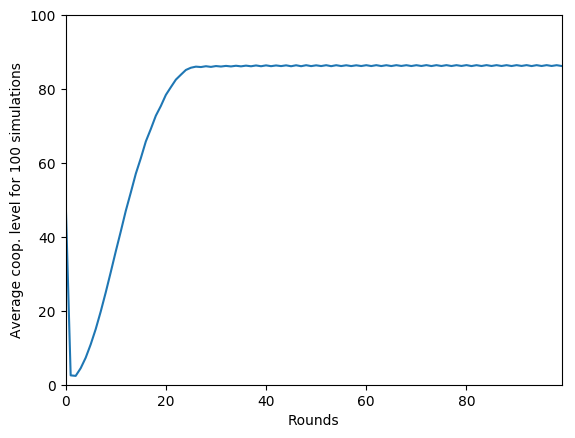
\includegraphics[width=1\linewidth]{images/assign2/50-part1}
        \caption{Moore neighborhood}
        \label{fig:50moorepart1}
    \end{subfigure}
    \begin{subfigure}{.5\textwidth}
        \centering
        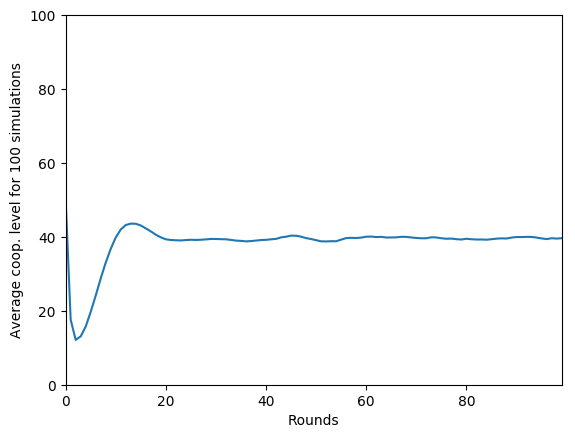
\includegraphics[width=1\linewidth]{images/assign2/50_vonneumann-part1}
        \caption{Von Neumann neigborhood}
        \label{fig:50vonpart1}
    \end{subfigure}
    \caption{Cooperation level using unconditional imitation and
    weak prisoner's dilemma on a 50x50 lattice.}
    \label{fig:50part1}
\end{figure}


\subsection{Lattice observation}

Figure \ref{fig:visu50part1} shows the full matrix of cooperation for
the rounds $t_{0}, t_{1}, t_{5}, t_{10}, t_{20}, t_{50}$. We can observe
that in the first round there is more or less the same number of players
cooperating and defecting. But in the second round, a large percentage
of players will choose to defect, leaving only smalls zone of cooperation.
This is due to the fact that a defecting player will usually have a better
score around a mixed neighborhood of player than a cooperating player.
But when a cooperating player has a cooperating neighborhood he will have
high enough score to influence defecting players in his neighborhood. We can
observe that in the following rounds, a sort of \textit{cluster} of cooperation
will be formed and influence the full lattice until reaching the cooperation
level explained in section \ref{neighborpart1}.

% Visualization for 50
\begin{figure}[H]
    \begin{subfigure}{.33\textwidth}
      \centering
      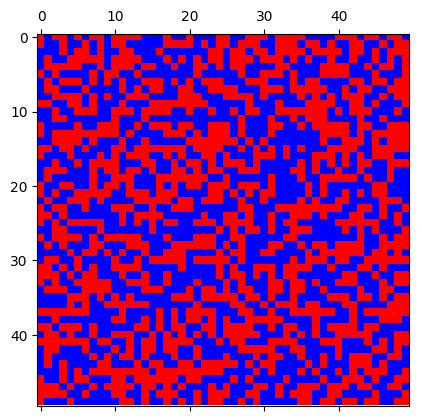
\includegraphics[width=1\linewidth]{images/assign2/visu_50-part1/t0}
      \caption{$t_0$}
      \label{fig:t0_50part1}
    \end{subfigure}
    \begin{subfigure}{.33\textwidth}
      \centering
      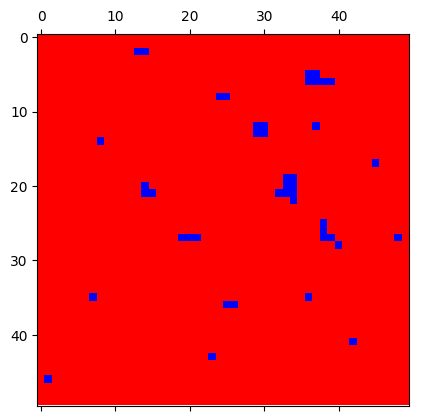
\includegraphics[width=1\linewidth]{images/assign2/visu_50-part1/t1}
      \caption{$t_1$}
      \label{fig:t1_50part1}
    \end{subfigure}
    \begin{subfigure}{.33\textwidth}
      \centering
      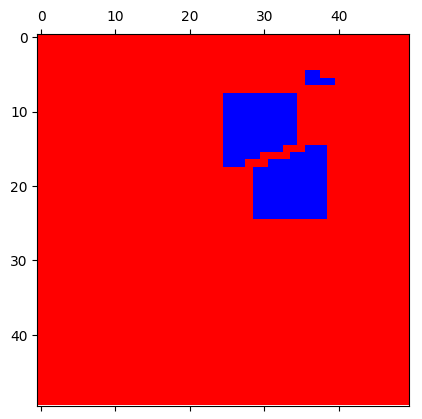
\includegraphics[width=1\linewidth]{images/assign2/visu_50-part1/t5}
      \caption{$t_5$}
      \label{fig:t5_50part1}
    \end{subfigure}
    \begin{subfigure}{.33\textwidth}
      \centering
      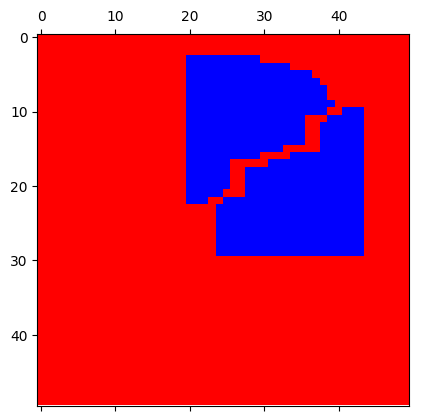
\includegraphics[width=1\linewidth]{images/assign2/visu_50-part1/t10}
      \caption{$t_{10}$}
      \label{fig:t10_50part1}
    \end{subfigure}
    \begin{subfigure}{.33\textwidth}
      \centering
      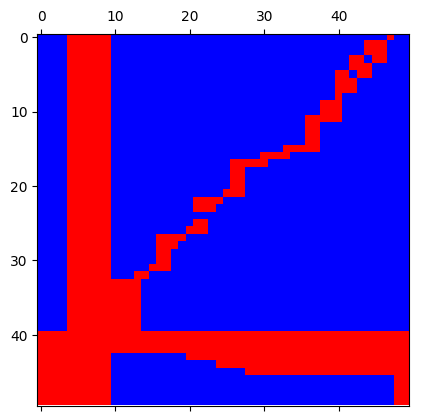
\includegraphics[width=1\linewidth]{images/assign2/visu_50-part1/t20}
      \caption{$t_{20}$}
      \label{fig:t20_50part1}
    \end{subfigure}
    \begin{subfigure}{.33\textwidth}
      \centering
      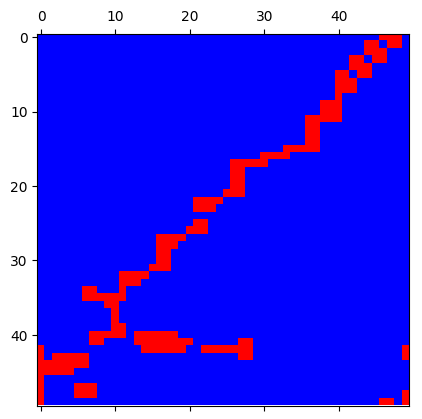
\includegraphics[width=1\linewidth]{images/assign2/visu_50-part1/t50}
      \caption{$t_{50}$}
      \label{fig:t50_50part1}
    \end{subfigure}
    \caption{Visualization of a the lattice with unconditional imitation,
    Moore neighborhood and weak prisoner's, dilemma.}
    \label{fig:visu50part1}
\end{figure}


\subsection{Lattice size analysis}

\paragraph{}

Figure \ref{fig:otherpart1}  shows the average cooperation level
of lattices of size 20, 12, 8 and 4. The behavior seems to the same
as in the analysis made against lattice of size 50
in section \ref{neighborpart1}, it crashes to a small level of cooperation
to grows and stabilize after a number of rounds. The plots show that when
the lattice size is small, the cooperation stabilize to a smaller cooperation
level than bigger lattices. We can observe that for a size 4 lattice,
the cooperation level is even 0 after the first round.

\paragraph{}

The reason could be that there is less players so less possibilities to
form some cooperation neighborhood, that will form the \texttt{clusters}
and grews as explained in previous section.


% Coop level for all others
\begin{figure}[H]
    \begin{subfigure}{.5\textwidth}
        \centering
        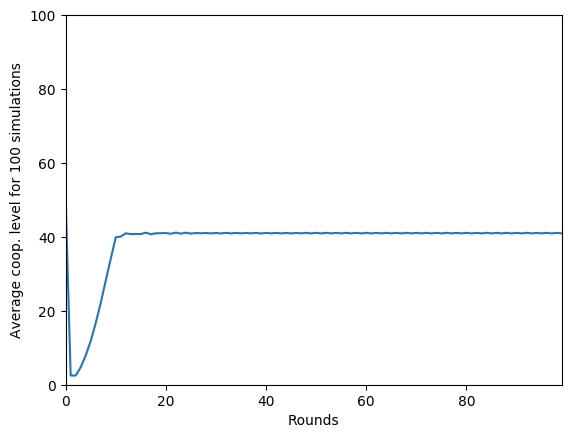
\includegraphics[width=1\linewidth]{images/assign2/20-part1}
        \caption{20x20}
        \label{fig:20moorepart1}
    \end{subfigure}
    \begin{subfigure}{.5\textwidth}
        \centering
        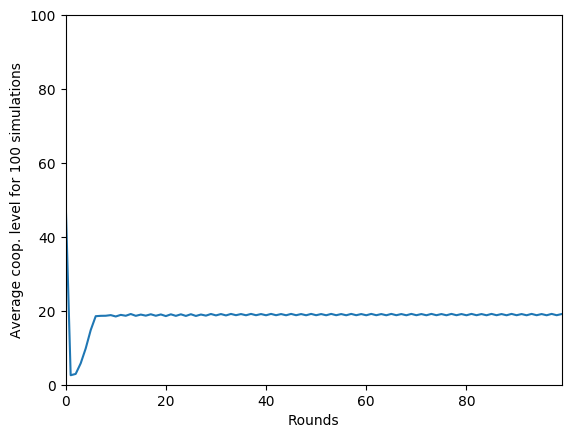
\includegraphics[width=1\linewidth]{images/assign2/12-part1}
        \caption{12x12}
        \label{fig:12moorepart1}
    \end{subfigure}
    \begin{subfigure}{.5\textwidth}
        \centering
        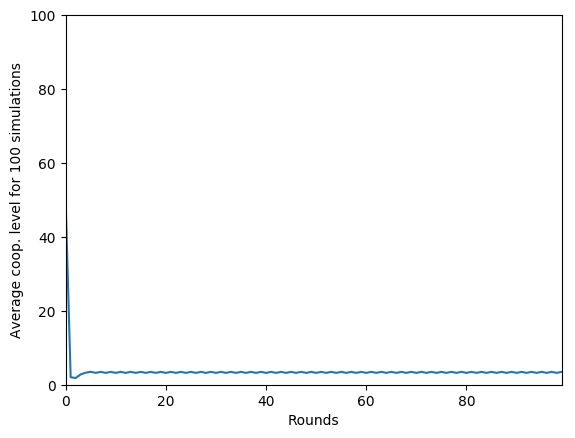
\includegraphics[width=1\linewidth]{images/assign2/8-part1}
        \caption{8x8}
        \label{fig:8moorepart1}
    \end{subfigure}
    \begin{subfigure}{.5\textwidth}
        \centering
        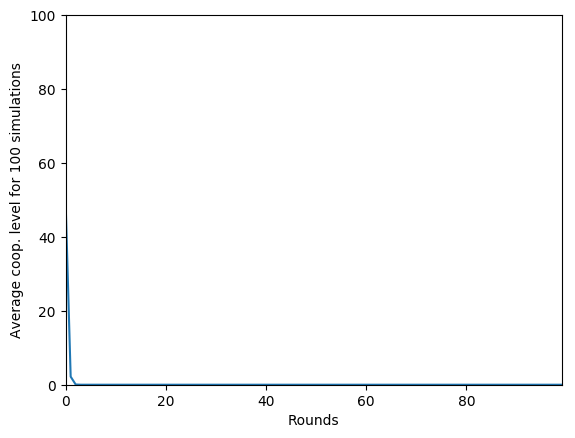
\includegraphics[width=1\linewidth]{images/assign2/4-part1}
        \caption{4x4}
        \label{fig:4moorepart1}
    \end{subfigure}
    \caption{Cooperation level using unconditional imitation, Moore neighborhood
    and weak prisoner's dilemma.}
    \label{fig:otherpart1}
\end{figure}

\section{Part II}

\subsection{Update mechanism}

\begin{equation}
    P_{ij} = (1 + [W_j - W_i] / [N\cdot(max\{P, R, T, S\}
    - min\{P, R, T, S\}])/2
\end{equation}

\paragraph{Intuitive observation}

This probabilty is interesting to be used as an update mechanism because
the probability to change the action to the neighbor action is
proportional to the difference between the players payoffs.

\paragraph{Probability variables}

$[W_j - W_i]$ is the difference between the two payoffs.
$N$ represent the number
of neighbor that the payoff calculation are based on. The difference
between the maximum and minimum multiply by $N$ is
the maximum payoff of a player. Since the payoffs cannot be bigger than
the maximum score, it is clear that $P_{ij}$ is a probability.

\paragraph{Analysis}

We can highlight different result from
the fration
$[W_j - W_i] / [N\cdot(max\{P, R, T, S\}
- min\{P, R, T, S\}]$
between the difference of payoffs and the maximum score:

\begin{enumerate}
    \item Fraction is positive when $W_j > W_i$. A special
    case is when $W_j$ is maximum and $W_i$ is null, the fraction is equal to 1.
    \item Fraction is negative when $W_i > W_j$. A special
    case is when $W_i$ is maximum and $W_j$ is null,
    the fraction is equal to -1.
    \item Fraction is equal to 0 when $W_i = W_j$
\end{enumerate}

By using the full definition of the probablity we can see that when in
case (1), it is more probable that the player will change is action
to the neighbor action, and sure if the fraction is equal 1
because $P_{ij} = 1$. When in (2),
it is more probable that the player will keep is action, and sure that
he will not change it when the fraction is equal to -1
because $P_{ij} = 0$. When in (3),
$P_{ij} = \frac{1}{2}$,
the payoff of the player and his neighbor are the same, which means that
both of their actions lead to the same payoff, so the probability to change
or to keep is the same.

\paragraph{Specifications}
Plots in Figure \ref{fig:50part2} shows the average cooperation level of 100
simulations with replicator rule as the update mechanism. The game played
is the snowdrift game.
The first rounds were played randomly,
where a player would choose cooperate with a probabilty of $\frac{1}{2}$.

\subsection{Neighborhood analysis}

\paragraph{Remark} The analysis is based on results from 50x50 lattice
simulations.

\paragraph{Moore}

Figure \ref{fig:50moorepart2} shows the average cooperation level using
the specifications above and a Moore neighborhood system.
In those simulations we can see that the cooperation
level drops at each round, but with a smaller factor over time.
%It is
%highly probable that when $t \rightarrow \infty$ the cooperation level
%tends to zero.
Here we see that around round 50, the cooperation level
is \textit{stable} at around 40\%. By \textit{stable} we mean that the
cooperation seems to drop lesser over time, but it still drops.

\paragraph{Von Neumann}


Figure \ref{fig:50vonpart2} shows the average cooperation level using
the specifications above and a Von Neumann neighborhood system. Even
with less neighbors per player, the pattern seems to be the same
than a Moore neighborhood over time.
It drops to be \textit{stable},
but with a far less cooperation level, around 20\%.
The difference between the Moore neighborhood is that the drop factor,
the lost of cooperation level over time, is bigger for a Von Neumann
neighborhood, and it takes more time to have a more \textit{stabilized}
cooperation level.

% Coop level for 50
\begin{figure}[H]
    \begin{subfigure}{.5\textwidth}
        \centering
        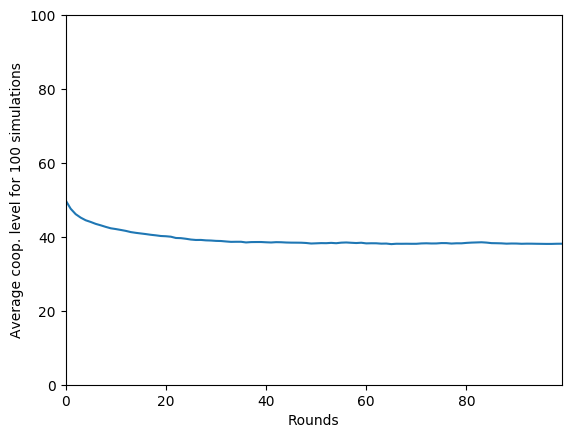
\includegraphics[width=1\linewidth]{images/assign2/50-part2}
        \caption{Moore neighborhood}
        \label{fig:50moorepart2}
    \end{subfigure}
    \begin{subfigure}{.5\textwidth}
        \centering
        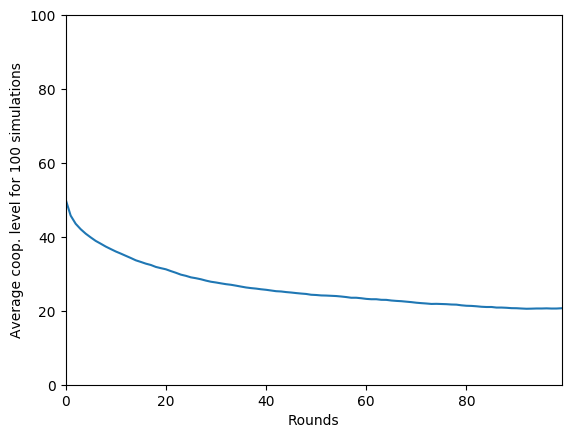
\includegraphics[width=1\linewidth]{images/assign2/50_vonneumann-part2}
        \caption{Von Neumann neigborhood}
        \label{fig:50vonpart2}
    \end{subfigure}
    \caption{Cooperation level using replicator rule and
    snowdrift game on a 50x50 lattice.}
    \label{fig:50part2}
\end{figure}

\paragraph{Comparaison with Part I}

In comparaison to Part I specifications and simulations, we see that her
the players seems to be less \textit{influenced} by their neighborhood.
This is due to the update mechanism. The replicator rule provide to the player
a way to respond to their neighborhood in a more \textit{intelligent} manner.
Indeed, when using the unconditional imitation, we saw that after the first
round the reactions of the players is extreme, a big majority of the players,
change their actions to defect, because in a equally distributed population,
defect usually have a better score. With the replicator rule each player,
based on his probability, will likely change his move only if it is
\textit{probably} better than his previous one.


\subsection{Lattice obseravion}

Figure \ref{fig:visu50part2} shows the evolution of the lattice over time.
In opposite the the lattice in Part I, her we see that the player are less
influenced by their neighborhood. Indeed, there is no form of
\textit{zone of cooperation}, that takes the advantage overtime.
We can see that overtime players tend to prefer to defect.

% Visualization for 50
\begin{figure}[H]
    \begin{subfigure}{.33\textwidth}
      \centering
      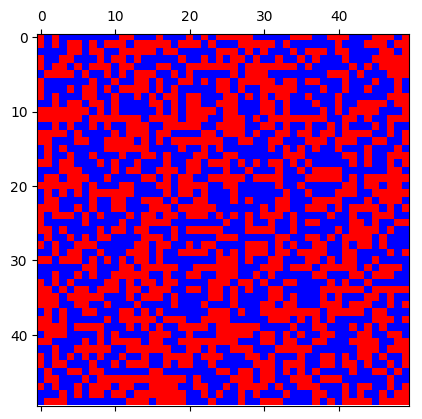
\includegraphics[width=1\linewidth]{images/assign2/visu_50-part2/t0}
      \caption{$t_0$}
      \label{fig:t0_50part2}
    \end{subfigure}
    \begin{subfigure}{.33\textwidth}
      \centering
      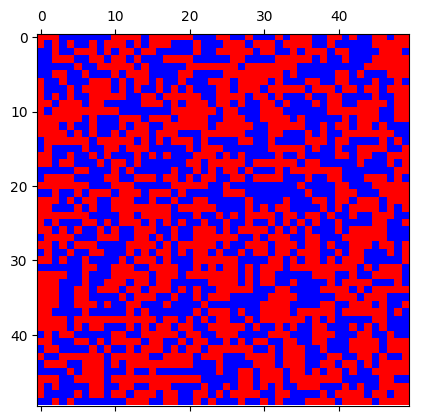
\includegraphics[width=1\linewidth]{images/assign2/visu_50-part2/t1}
      \caption{$t_1$}
      \label{fig:t1_50part2}
    \end{subfigure}
    \begin{subfigure}{.33\textwidth}
      \centering
      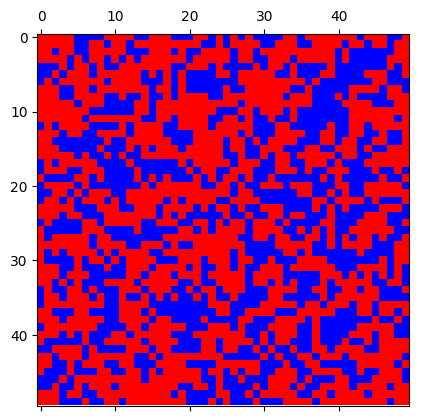
\includegraphics[width=1\linewidth]{images/assign2/visu_50-part2/t5}
      \caption{$t_5$}
      \label{fig:t5_50part2}
    \end{subfigure}
    \begin{subfigure}{.33\textwidth}
      \centering
      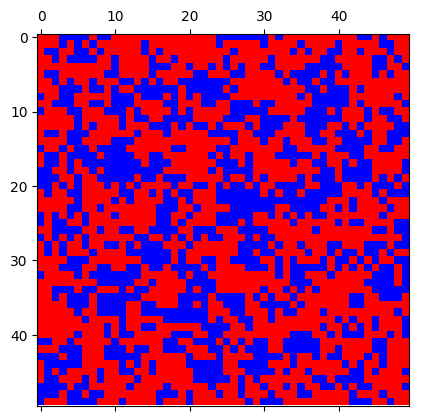
\includegraphics[width=1\linewidth]{images/assign2/visu_50-part2/t10}
      \caption{$t_{10}$}
      \label{fig:t10_50part2}
    \end{subfigure}
    \begin{subfigure}{.33\textwidth}
      \centering
      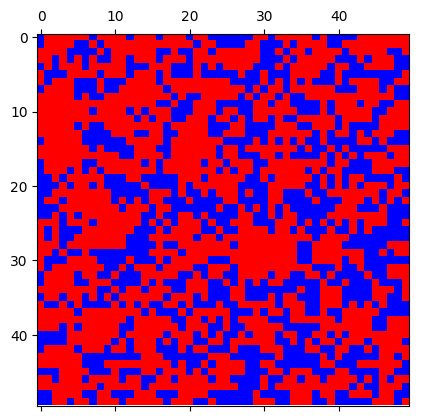
\includegraphics[width=1\linewidth]{images/assign2/visu_50-part2/t20}
      \caption{$t_{20}$}
      \label{fig:t20_50part2}
    \end{subfigure}
    \begin{subfigure}{.33\textwidth}
      \centering
      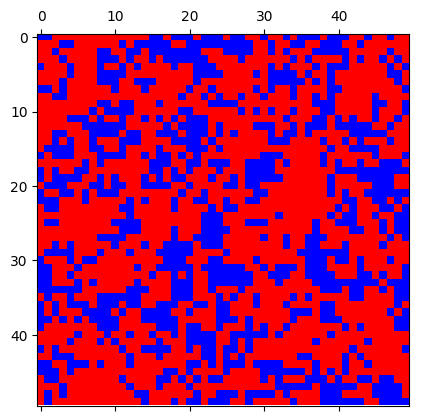
\includegraphics[width=1\linewidth]{images/assign2/visu_50-part2/t50}
      \caption{$t_{50}$}
      \label{fig:t50_50part2}
    \end{subfigure}
    \caption{Visualization of a the lattice with replicator rule,
    Moore neighborhood and snowdrift game.}
    \label{fig:visu50part2}
\end{figure}

\subsection{Lattice size analysis}

Figure \ref{fig:otherpart2} shows the cooperation level for matrix of
different size. The pattern here is the same for the lattice 50x50. The
cooperation level drops over time to be \textit{steady} at around 40\%.
Except for the lattice of size 4 where the cooperation level drops more and
it is smaller that for the other size. We can suppose that here when the
lattice is too small, and the probability of cooperate in a smaller lattice
is smaller that with bigger lattice. In conclusion, we can see that for
this specifications,
size does not matter, up to a point where the lattice is too small,
in opposite of specifications of Part I, where the behaviour is different
with lattice of different size.

% Coop level for all others
\begin{figure}[H]
    \begin{subfigure}{.5\textwidth}
        \centering
        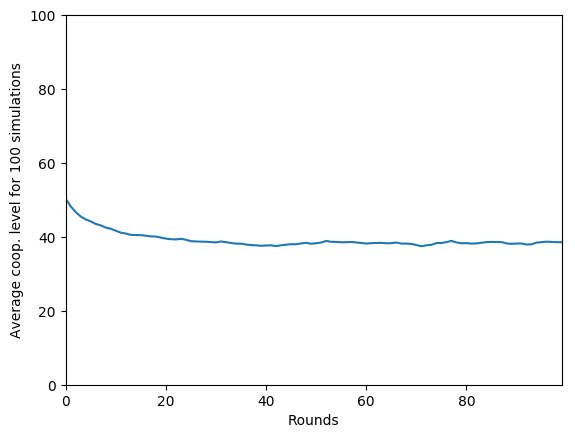
\includegraphics[width=1\linewidth]{images/assign2/20-part2}
        \caption{20x20}
        \label{fig:20moorepart2}
    \end{subfigure}
    \begin{subfigure}{.5\textwidth}
        \centering
        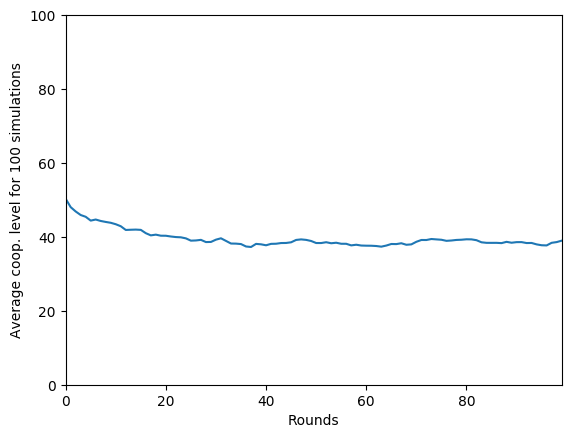
\includegraphics[width=1\linewidth]{images/assign2/12-part2}
        \caption{12x12}
        \label{fig:12moorepart2}
    \end{subfigure}
    \begin{subfigure}{.5\textwidth}
        \centering
        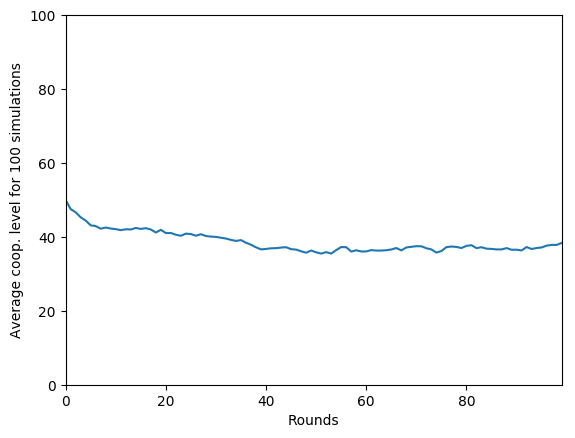
\includegraphics[width=1\linewidth]{images/assign2/8-part2}
        \caption{8x8}
        \label{fig:8moorepart2}
    \end{subfigure}
    \begin{subfigure}{.5\textwidth}
        \centering
        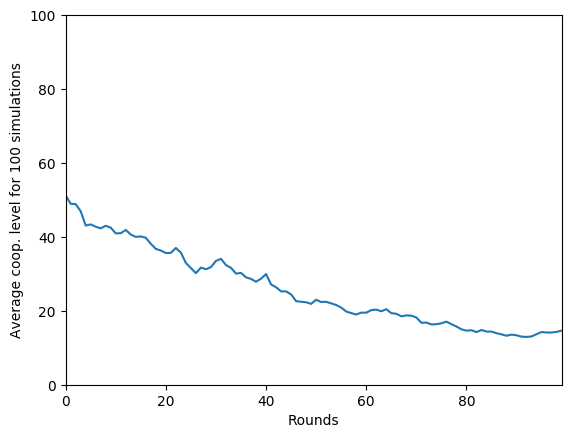
\includegraphics[width=1\linewidth]{images/assign2/4-part2}
        \caption{4x4}
        \label{fig:4moorepart2}
    \end{subfigure}
    \caption{Cooperation level using replicator rule, Moore neighborhood
    and snowdrift game}
    \label{fig:otherpart2}
\end{figure}


\section{Part III}

\subsection{Specifications}


In this part we will discuss the behaviour of the same mechanics used
in sections above but by changing the start round population. The idea is the
following: a zone in the center that is equally distributed
between cooperation and defection, i.e. a random start round for the
players in the center, and this population be surrounded by
full cooperation or full defection players. We will ask two questions:
How the cooperation level changes over time, and is the final results
identical as in Part I and Part II.

\subsection{Results}

\paragraph{Remark} The simulations were run on a 50x50 lattice, with
a 10x10 \textit{center zone} and 300 rounds played.

\subsubsection{Part I mechanisms}

\begin{figure}[H]
    \begin{subfigure}{.5\textwidth}
        \centering
        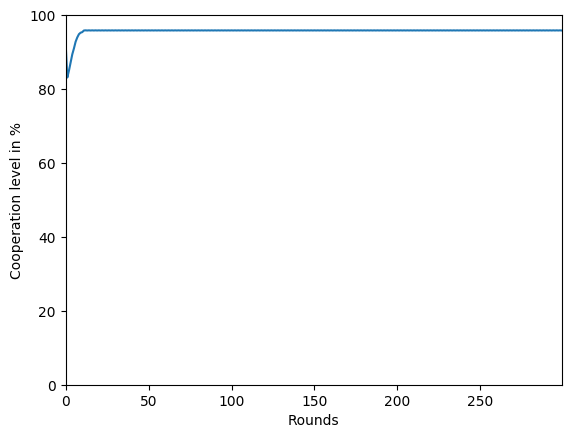
\includegraphics[width=1\linewidth]{images/assign2/part31-coop/coop.png}
        \caption{Cooperation surrounding}
        \label{fig:part31-coop}
    \end{subfigure}
    \begin{subfigure}{.5\textwidth}
        \centering
        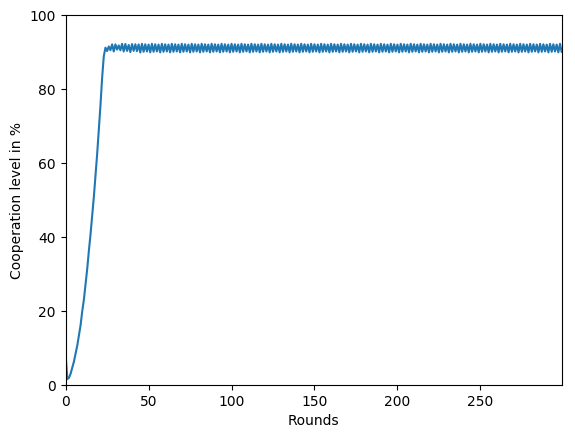
\includegraphics[width=1\linewidth]
        {images/assign2/part31-defect/coop.png}
        \caption{Defection surrounding}
        \label{fig:part31-defect}
    \end{subfigure}
    \caption{Cooperation level using unconditional imitation and
    weak prisoner's dilemma on a 50x50 lattice and 10x10 center zone.}
    \label{fig:50part1}
\end{figure}


\paragraph{Cooperation surrounding}

\label{part31-coop}

Figure \ref{fig:part31-coop} shows
the cooperation level when using the same configuration as Part I
with a Moore neighborhood, with the center zone surrounded
by cooperation players. Figure \ref{fig:visupart31-coop} shows the
lattice of this simulation over time. We can see that in this simulation
the surrounded players are not affected by the center zone (except for the
closest players). Indeed the behaviour is as explained in Part I, the
cooperation level drops to a very low rate, and form a cluster that will
take advantage over time and \textit{stabilize} around 95\%. This percentage
is higher than in Part I because the cooperation level changes only
in the center zone.

% part31-coop
\begin{figure}[H]
    \begin{subfigure}{.33\textwidth}
      \centering
      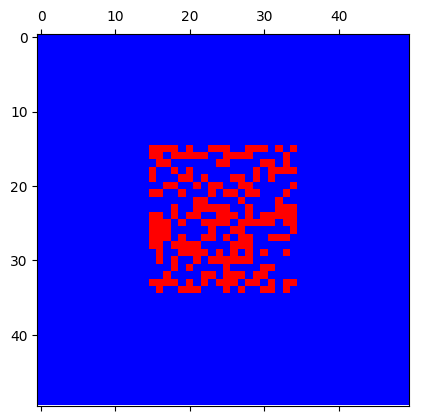
\includegraphics[width=1\linewidth]{images/assign2/part31-coop/t0}
      \caption{$t_{0}$}
    \end{subfigure}
    \begin{subfigure}{.33\textwidth}
      \centering
      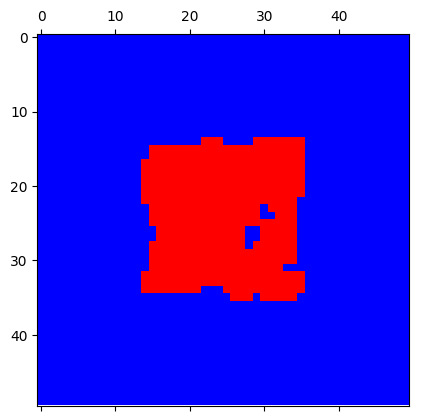
\includegraphics[width=1\linewidth]{images/assign2/part31-coop/t1}
      \caption{$t_{1}$}
    \end{subfigure}
    \begin{subfigure}{.33\textwidth}
      \centering
      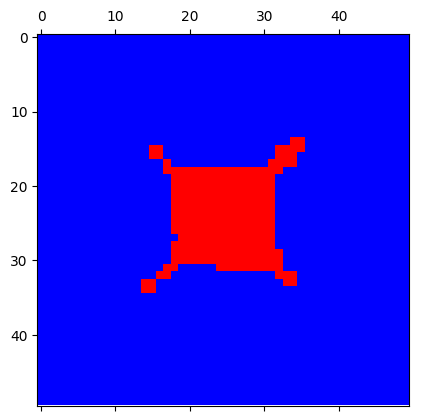
\includegraphics[width=1\linewidth]{images/assign2/part31-coop/t5}
      \caption{$t_{5}$}
    \end{subfigure}
    \begin{subfigure}{.33\textwidth}
      \centering
      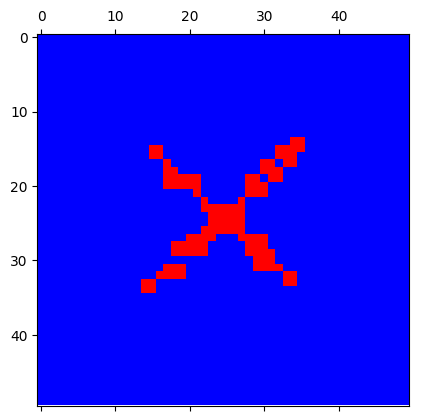
\includegraphics[width=1\linewidth]{images/assign2/part31-coop/t10}
      \caption{$t_{10}$}
    \end{subfigure}
    \begin{subfigure}{.33\textwidth}
      \centering
      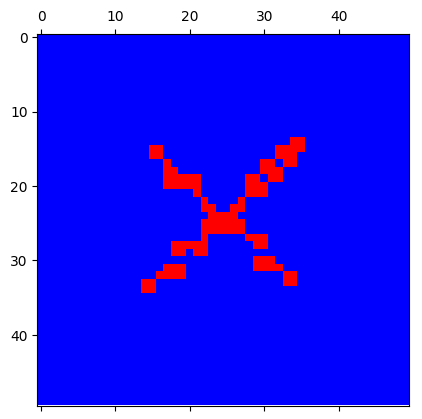
\includegraphics[width=1\linewidth]{images/assign2/part31-coop/t20}
      \caption{$t_{20}$}
    \end{subfigure}
    \begin{subfigure}{.33\textwidth}
      \centering
      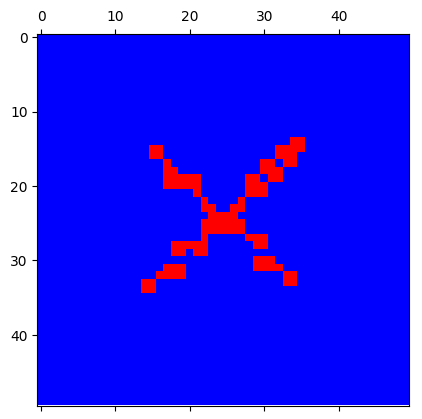
\includegraphics[width=1\linewidth]{images/assign2/part31-coop/t40}
      \caption{$t_{40}$}
    \end{subfigure}
    \begin{subfigure}{.33\textwidth}
      \centering
      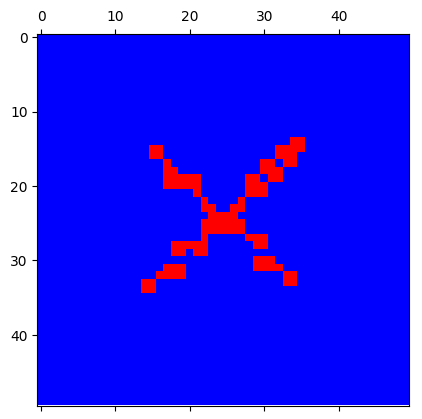
\includegraphics[width=1\linewidth]{images/assign2/part31-coop/t50}
      \caption{$t_{50}$}
    \end{subfigure}
    \begin{subfigure}{.33\textwidth}
      \centering
      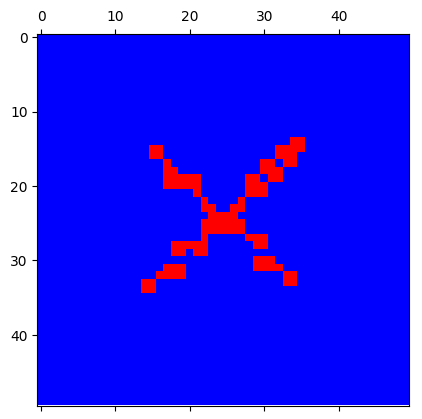
\includegraphics[width=1\linewidth]{images/assign2/part31-coop/t60}
      \caption{$t_{60}$}
    \end{subfigure}
    \begin{subfigure}{.33\textwidth}
      \centering
      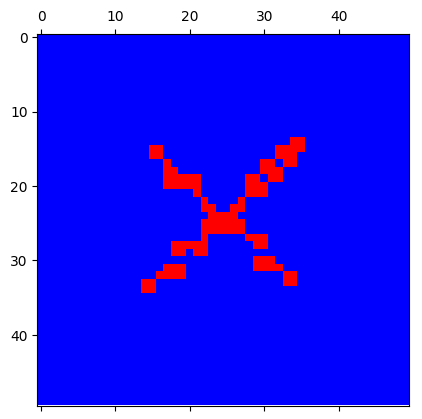
\includegraphics[width=1\linewidth]{images/assign2/part31-coop/t100}
      \caption{$t_{100}$}
    \end{subfigure}
    \caption{Visualization of the lattice with unconditional imitation,
    Moore neighborhood and weak prisoner's, dilemma. The start round is
    a 10x10 center zone and surrounded by cooperation players.}
    \label{fig:visupart31-coop}
\end{figure}

\paragraph{Defection surrounding}

Figure \ref{fig:part31-defect} shows
the cooperation level when using the same configuration as Part I
with a Moore neighborhood, with the center zone surrounded
by defecting players. Figure \ref{fig:visupart31-defect} shows the
lattice of this simulation over time. Here we can see that the center zone
influenced the surrounding population. As soon as the cluster are formed
in the center zone, the cooperation level grows up to \textit{stabilize}
at around 90\%. Here the cooperation level is more or less the same
as exposed in Part I, because in $t_1$, the defecting
players are a majority, as
opposed to cooperation surrounding where only the center zone has a majority
of defecting players.

% part31-defect
\begin{figure}[H]
    \begin{subfigure}{.33\textwidth}
      \centering
      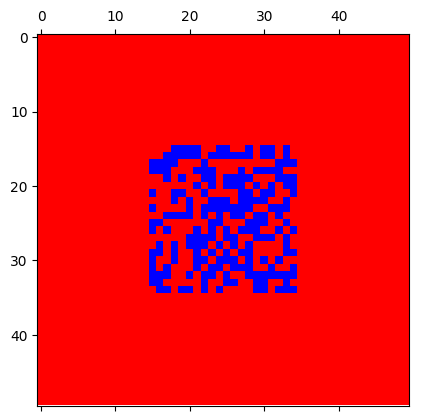
\includegraphics[width=1\linewidth]{images/assign2/part31-defect/t0}
      \caption{$t_{0}$}
    \end{subfigure}
    \begin{subfigure}{.33\textwidth}
      \centering
      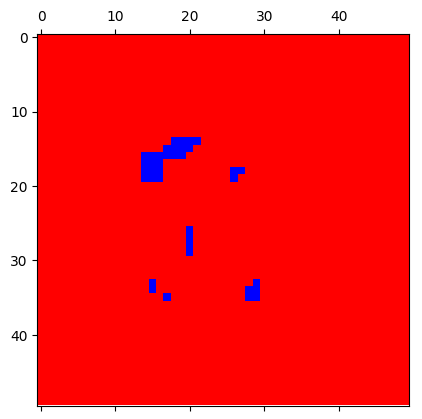
\includegraphics[width=1\linewidth]{images/assign2/part31-defect/t1}
      \caption{$t_{1}$}
    \end{subfigure}
    \begin{subfigure}{.33\textwidth}
      \centering
      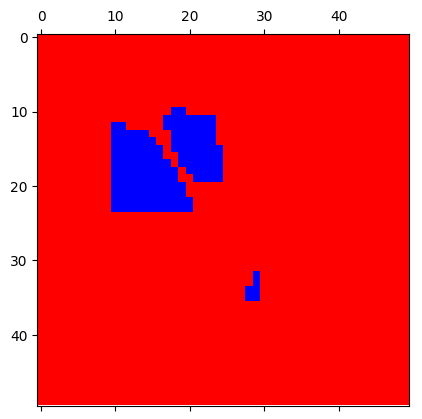
\includegraphics[width=1\linewidth]{images/assign2/part31-defect/t5}
      \caption{$t_{5}$}
    \end{subfigure}
    \begin{subfigure}{.33\textwidth}
      \centering
      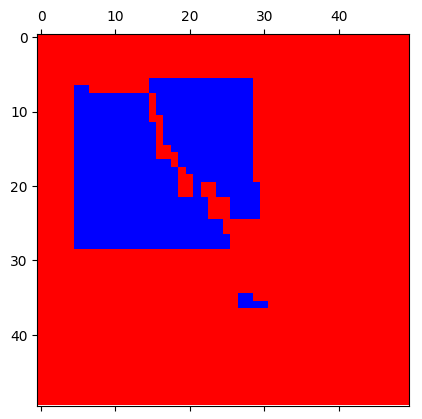
\includegraphics[width=1\linewidth]{images/assign2/part31-defect/t10}
      \caption{$t_{10}$}
    \end{subfigure}
    \begin{subfigure}{.33\textwidth}
      \centering
      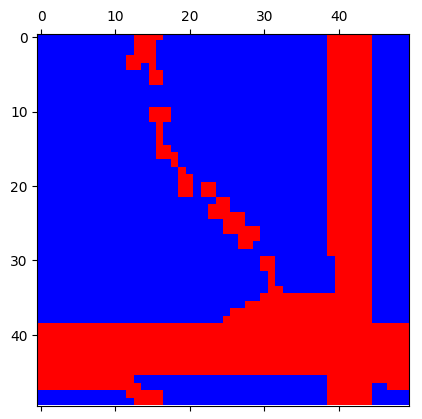
\includegraphics[width=1\linewidth]{images/assign2/part31-defect/t20}
      \caption{$t_{20}$}
    \end{subfigure}
    \begin{subfigure}{.33\textwidth}
      \centering
      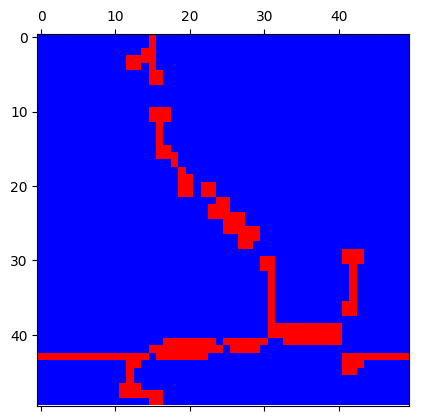
\includegraphics[width=1\linewidth]{images/assign2/part31-defect/t40}
      \caption{$t_{40}$}
    \end{subfigure}
    \begin{subfigure}{.33\textwidth}
      \centering
      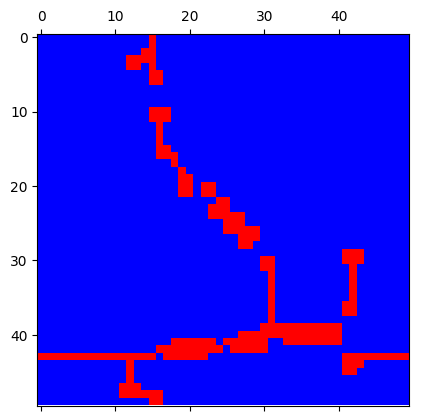
\includegraphics[width=1\linewidth]{images/assign2/part31-defect/t50}
      \caption{$t_{50}$}
    \end{subfigure}
    \begin{subfigure}{.33\textwidth}
      \centering
      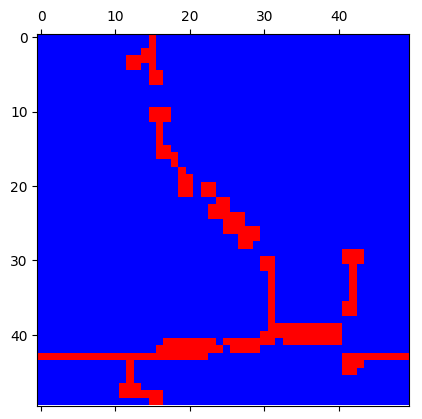
\includegraphics[width=1\linewidth]{images/assign2/part31-defect/t60}
      \caption{$t_{60}$}
    \end{subfigure}
    \begin{subfigure}{.33\textwidth}
      \centering
      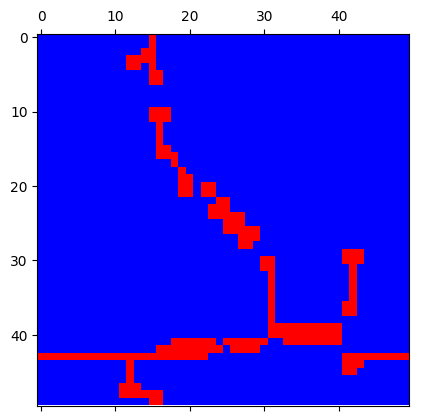
\includegraphics[width=1\linewidth]{images/assign2/part31-defect/t100}
      \caption{$t_{100}$}
    \end{subfigure}
    \caption{Visualization of a the lattice with unconditional imitation,
    Moore neighborhood and weak prisoner's, dilemma. The start round is
    a 10x10 center zone and surrounded by defection players.}
    \label{fig:visupart31-defect}
\end{figure}


\subsubsection{Part II mechanisms}

\begin{figure}[H]
    \begin{subfigure}{.5\textwidth}
        \centering
        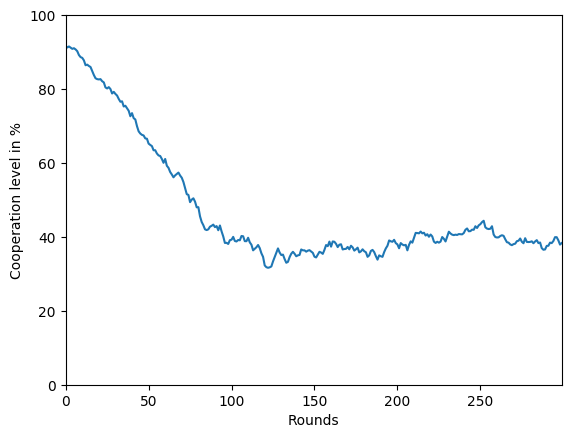
\includegraphics[width=1\linewidth]
        {images/assign2/part32-coop/coop.png}
        \caption{Cooperation surrounding}
        \label{fig:part32-coop}
    \end{subfigure}
    \begin{subfigure}{.5\textwidth}
        \centering
        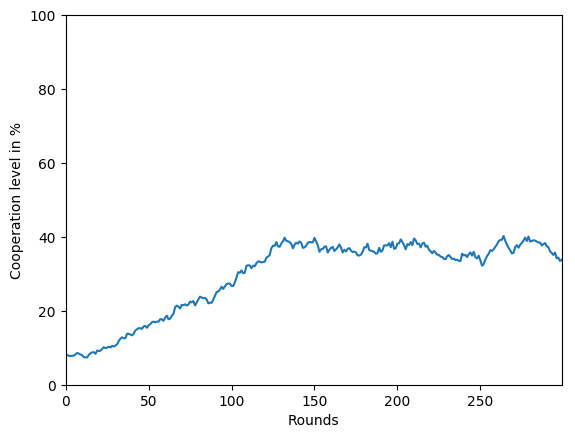
\includegraphics[width=1\linewidth]
        {images/assign2/part32-defect/coop.png}
        \caption{Defection surrounding}
        \label{fig:part32-defect}
    \end{subfigure}
    \caption{Cooperation level using replicator rule and
    snowdrift game on a 50x50 lattice and 10x10 center zone.}
    \label{fig:50part2}
\end{figure}

\paragraph{Cooperation surrounding}

Figure \ref{fig:part32-coop} shows
the cooperation level when using the same configuration as Part II
with a Moore neighborhood, with the center zone surrounded
by cooperation players. Figure \ref{fig:visupart32-coop} shows the
lattice of this simulation over time. The cooperation level over time
is decreasing until reaching a level around 40\%. As shown in the visualization
we see that the surrounding cooperating players are influenced by the center
zone players. Indeed, players close to the center zone are changing their
actions based on the results of the center players score. We can see
that at round $t_{100}$, the full population has been influenced
by the results of the center zone games, and the distribution of
players seems identical
to the results exposed in Part II, the cooperation is \textit{stabilize}
at around 40\%. As opposed to cooperation surrounding
in section \ref{part31-coop}, here the full population is influenced and
change their actions, where in the cooperation surrounding using Part I
mechanisms the players stick to their cooperating action.

% part32-coop
\begin{figure}[H]
    \begin{subfigure}{.33\textwidth}
      \centering
      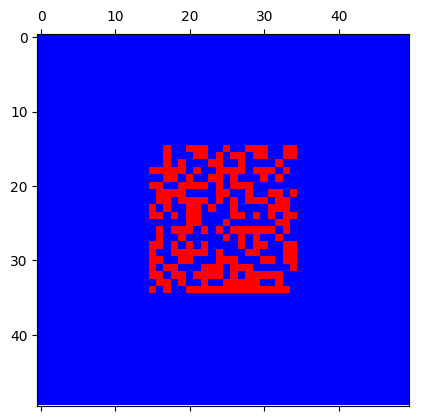
\includegraphics[width=1\linewidth]{images/assign2/part32-coop/t0}
      \caption{$t_{0}$}
    \end{subfigure}
    \begin{subfigure}{.33\textwidth}
      \centering
      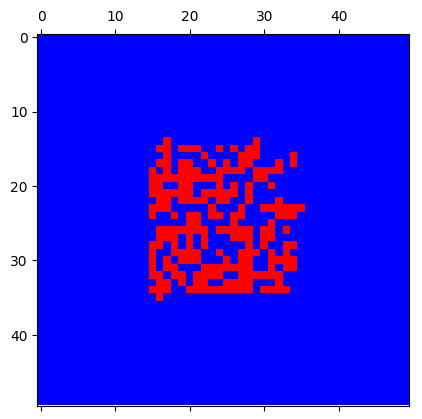
\includegraphics[width=1\linewidth]{images/assign2/part32-coop/t1}
      \caption{$t_{1}$}
    \end{subfigure}
    \begin{subfigure}{.33\textwidth}
      \centering
      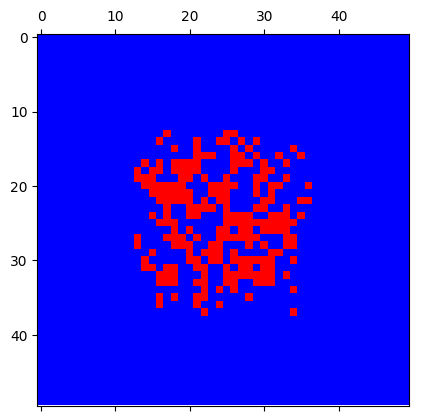
\includegraphics[width=1\linewidth]{images/assign2/part32-coop/t5}
      \caption{$t_{5}$}
    \end{subfigure}
    \begin{subfigure}{.33\textwidth}
      \centering
      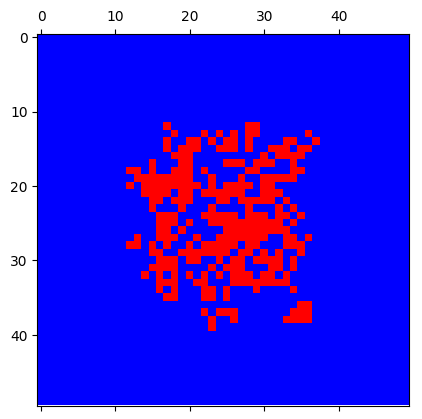
\includegraphics[width=1\linewidth]{images/assign2/part32-coop/t10}
      \caption{$t_{10}$}
    \end{subfigure}
    \begin{subfigure}{.33\textwidth}
      \centering
      \includegraphics[width=1\linewidth]{images/assign2/part32-coop/t20}
      \caption{$t_{20}$}
    \end{subfigure}
    \begin{subfigure}{.33\textwidth}
      \centering
      \includegraphics[width=1\linewidth]{images/assign2/part32-coop/t40}
      \caption{$t_{40}$}
    \end{subfigure}
    \begin{subfigure}{.33\textwidth}
      \centering
      \includegraphics[width=1\linewidth]{images/assign2/part32-coop/t50}
      \caption{$t_{50}$}
    \end{subfigure}
    \begin{subfigure}{.33\textwidth}
      \centering
      \includegraphics[width=1\linewidth]{images/assign2/part32-coop/t60}
      \caption{$t_{60}$}
    \end{subfigure}
    \begin{subfigure}{.33\textwidth}
      \centering
      \includegraphics[width=1\linewidth]{images/assign2/part32-coop/t100}
      \caption{$t_{100}$}
    \end{subfigure}
    \caption{Visualization of a the lattice with replicator rule,
    Moore neighborhood and weak snowdrift game. The start round is
    a 10x10 center zone and surrounded by cooperation players.}
    \label{fig:visupart32-coop}
\end{figure}


\paragraph{Defection surrounding}

Figure \ref{fig:part32-defect} shows
the cooperation level when using the same configuration as Part II
with a Moore neighborhood, with the center zone surrounded
by defecting players. Figure \ref{fig:visupart32-defect} shows the
lattice of this simulation over time. The pattern seems to be the same
as exposed in cooperation surrounding. The center zone, influenced
the players close to the them, until it reaches the full population.
Here the cooperation level is low, since cooperating players can only be
found in the center zone in the first round.
It is growing over time to reach a \textit{stabilize}
state at around 40\% which.

% part32-defect
\begin{figure}[H]
    \begin{subfigure}{.33\textwidth}
      \centering
      \includegraphics[width=1\linewidth]{images/assign2/part32-defect/t0}
      \caption{$t_{0}$}
    \end{subfigure}
    \begin{subfigure}{.33\textwidth}
      \centering
      \includegraphics[width=1\linewidth]{images/assign2/part32-defect/t1}
      \caption{$t_{1}$}
    \end{subfigure}
    \begin{subfigure}{.33\textwidth}
      \centering
      \includegraphics[width=1\linewidth]{images/assign2/part32-defect/t5}
      \caption{$t_{5}$}
    \end{subfigure}
    \begin{subfigure}{.33\textwidth}
      \centering
      \includegraphics[width=1\linewidth]{images/assign2/part32-defect/t10}
      \caption{$t_{10}$}
    \end{subfigure}
    \begin{subfigure}{.33\textwidth}
      \centering
      \includegraphics[width=1\linewidth]{images/assign2/part32-defect/t20}
      \caption{$t_{20}$}
    \end{subfigure}
    \begin{subfigure}{.33\textwidth}
      \centering
      \includegraphics[width=1\linewidth]{images/assign2/part32-defect/t40}
      \caption{$t_{40}$}
    \end{subfigure}
    \begin{subfigure}{.33\textwidth}
      \centering
      \includegraphics[width=1\linewidth]{images/assign2/part32-defect/t50}
      \caption{$t_{50}$}
    \end{subfigure}
    \begin{subfigure}{.33\textwidth}
      \centering
      \includegraphics[width=1\linewidth]{images/assign2/part32-defect/t60}
      \caption{$t_{60}$}
    \end{subfigure}
    \begin{subfigure}{.33\textwidth}
      \centering
      \includegraphics[width=1\linewidth]{images/assign2/part32-defect/t100}
      \caption{$t_{100}$}
    \end{subfigure}
    \caption{Visualization of a the lattice with replicator rule,
    Moore neighborhood and weak snowdrift game. The start round is
    a 10x10 center zone and surrounded by defecting players.}
    \label{fig:visupart32-defect}
\end{figure}


\end{document}
